% IEEE Geoscience and Remote Sensing Letters
% 5-page limit (4 pages + 1 page of references).
%
% Build:   latexmk -pdf whirlwind3d.tex
% Cleanup: latexmk -c
%
% Template based on the official IEEE GRSL template
% https://www.overleaf.com/latex/templates/ieee-geoscience-and-remote-sensing-letters-official-ieee-latex-template/zckwcmrxbvhg
% (IEEEtran class with \documentclass[journal]{IEEEtran}; standard packages).

\documentclass[journal]{IEEEtran}

\usepackage{amsmath,amssymb,amsfonts}
\usepackage{graphicx}
\usepackage{booktabs}
\usepackage{xcolor}
\usepackage[colorlinks=true,linkcolor=black,citecolor=black,urlcolor=blue]{hyperref}
\usepackage{cite}

\graphicspath{{figures/}}

% Hyphenation handles for tricky words
\hyphenation{whirl-wind un-wrap-ping phase-link-ed Pa-los Ver-des}

\begin{document}

\title{Closure-Aware Phase Unwrapping of Phase-Linked InSAR Time Series\\
       with CRLB-Weighted Cost and Boundary-Aware Residues}

\author{Scott Staniewicz%
\thanks{S. Staniewicz is with the University of Texas at Austin
        (e-mail: scott.stanie@utexas.edu).}%
\thanks{Manuscript submitted \today.}%
}

\markboth{IEEE Geoscience and Remote Sensing Letters, vol.~XX, no.~Y, 20ZZ}%
{Staniewicz: Closure-Aware Phase Unwrapping of Phase-Linked InSAR Time Series}

\maketitle

% --- Abstract -------------------------------------------------------------

\begin{abstract}
Multi-temporal InSAR pipelines that estimate per-acquisition phase via phase
linking emit, alongside each interferogram (IG), a per-pixel
Cram\'er--Rao Lower Bound (CRLB) raster that is a tighter per-pixel
noise model than the sliding-window sample coherence used by classical
unwrappers. We exploit this in two ways. First, the per-IG 2D unwrap uses
a CRLB-weighted Bayesian arc cost in place of the Lee-coherence cost.
Second, the wrapped-phase identity around any temporal cycle
$\sum_e\varepsilon_e\psi_e\equiv 0\,(\bmod 2\pi)$ - guaranteed exactly by
phase linking - turns the residual integer cycle counts into an
\emph{exact} per-pixel reliability metric. A correctness bug in the
residue-grid boundary handling of the underlying 2D unwrapper is
diagnosed and fixed: wrap-lines exiting at an image edge had no node to
terminate on, so MCF was forced to pair them with distant interior
partners and integration along the snake path picked up wildly wrong
integer counts. With the fix, our Rust implementation
(\texttt{whirlwind-rs}) agrees with dolphin's SNAPHU output at 100\%
of pixels modulo $2\pi$ on every one of 150 IGs over a Palos Verdes
$4065\times 3802$ stack, with median absolute per-IG RMS of 2.31~rad
(versus 4.72~rad without the fix). We also describe a tiled mode that
matches the non-tiled output at 99.78\% of pixels at $2\times$ wall-clock
and a virtual ground-node MCF variant that fixes the unit-capacity
limitation on boundary-bound wrap-lines.
\end{abstract}

\begin{IEEEkeywords}
Synthetic aperture radar, interferometry, phase unwrapping, time-series
analysis, phase linking, minimum cost flow, Cram\'er--Rao Lower Bound.
\end{IEEEkeywords}

% --- Sections -------------------------------------------------------------

\section{Introduction}\label{sec:intro}

\IEEEPARstart{P}{hase} unwrapping for InSAR time series has been treated in
two largely disjoint ways: either as $N(N-1)/2$ independent 2D problems
(unwrap each IG separately with SNAPHU \cite{snaphu}, PHASS, etc., and
accept the per-IG inconsistencies) or as a separable temporal-then-spatial
problem (e.g.\ spurt's EMCF \cite{spurt}). Neither exploits the
fact that phase-linked IGs \cite{phaselink-emi,phaselink-evd} live in a
$(D-1)$-dimensional subspace of per-acquisition phases, with
the wrapped-phase identity
\begin{equation}
\sum_{e\in C} \varepsilon_e\,\psi_e \;\equiv\; 0 \pmod{2\pi}
\label{eq:closure}
\end{equation}
holding \emph{exactly} for every closed cycle $C$ in the temporal graph
(where $\varepsilon_e\in\{\pm 1\}$ is the orientation of edge $e$ in
$C$). The unwrap problem then reduces to integer-ambiguity estimation:
find $k_e\in\mathbb{Z}$ per IG such that
\begin{equation}
\psi_e = \tilde\psi_e + 2\pi k_e
\end{equation}
satisfies \eqref{eq:closure} exactly, with the per-pixel noise model
coming from CRLB rather than sample coherence. This is structurally the
GNSS / LAMBDA carrier-phase ambiguity-resolution problem \cite{lambda}.

This letter (i) replaces the classical Lee-coherence arc cost of the
underlying 2D MCF unwrapper \cite{carballo,whirlwind} with a
CRLB-weighted Gaussian cost; (ii) identifies and fixes a residue-grid
boundary bug in the standard formulation that silently dropped
wrap-line endpoints at the image edges, with severe practical
consequences on real data; (iii) introduces a per-pixel quality map
derived directly from the temporal closure residual that, because of
phase linking's exact closure guarantee, is integer-valued and
interpretable as a wrap-mistake count; (iv) describes a tile-and-stitch
mode that bounds per-IG memory; and (v) describes a virtual ground-node
MCF variant that fixes the unit-capacity limitation of the basic MCF
for boundary-bound wrap-lines.

% --- Method ---------------------------------------------------------------

\section{Method}\label{sec:method}

\subsection{Per-IG 2D unwrap with CRLB cost}\label{sec:crlb-cost}

Let $\sigma^2_e(p)=\sigma^2_a(p)+\sigma^2_b(p)$ be the per-IG phase
variance at pixel $p$, with $\sigma^2_a$, $\sigma^2_b$ read from the
per-acquisition CRLB rasters phase linking emits \cite{phaselink-emi}.
We assign the per-arc cost in the MCF residue graph as
\begin{equation}
c(\alpha,\sigma^2_{\rm arc}) \;=\; \frac{1}{\sigma^2_{\rm arc}}\cdot
\max(0,\pi-|\alpha|),
\label{eq:crlbcost}
\end{equation}
with $\sigma^2_{\rm arc}=\sigma^2_e(p)+\sigma^2_e(q)$ summed over the
two endpoint pixels of the arc and $\alpha$ the smoothed local phase
gradient. The shape $\pi-|\alpha|$ keeps the MCF tractable
(non-negative reduced costs); the $1/\sigma^2$ prefactor is the Fisher
information for the gradient. A CRLB-nodata sentinel (the per-pixel
value $0$ that phase linking writes for pixels that did not pass
PS/DS selection) maps to a large $\sigma^2_{\rm nodata}\approx 50$
rad${}^2$ so MCF can route flow freely through unreliable pixels
without treating them as ``essentially noiseless''.

\subsection{Residue-grid boundary handling}\label{sec:bdy}

The textbook 2D-MCF unwrapper computes residues from $2\times 2$
plaquettes interior to the image. Partial plaquettes at the four image
edges are typically dropped (zeroed), implicitly asserting that no
wrap-line exits the image. On real data with high residue density,
this assertion is wrong: wrap-lines do exit at every image edge, and
without a residue at the exit point MCF is forced to pair each interior
endpoint with an opposite-sign \emph{interior} partner. The flow then
takes long internal paths instead of the actual wrap-line path; in
particular, snake-path integration along column~0 picks up large
cumulative integer counts and the unwrapped output exhibits striped
$\pm 2\pi$ jumps across rows.

The fix is to compute residues along all four boundary edges using
one-sided $\mathrm{cycle\_diff}$ and signs chosen so that, by Stokes's
theorem, the augmented residue grid is globally charge-balanced
($\sum_p r(p)\equiv 0$). MCF then drains wrap-line termination charge
through the cost-0 frame-along arcs without injecting spurious
corrections into the interior. Fig.~\ref{fig:bdyfix} compares the
unwrapped output before and after the fix on a Palos Verdes 1024²
tile.

\subsection{Per-pixel reliability from closure residual}\label{sec:quality}

After per-IG 2D unwrap, the cycle sum for any closed temporal cycle is,
by \eqref{eq:closure},
$\sum_e\varepsilon_e\psi_e(p) = 2\pi K_C(p)$ with $K_C(p)\in\mathbb{Z}$
\emph{exactly}. We define the per-pixel quality $Q(p)$ as
\begin{equation}
Q(p) \;=\; \max_{C\in\mathcal{T}}|K_C(p)|,
\end{equation}
where $\mathcal{T}$ is the set of all temporal triangles
(3-cycles). $Q=0$ means every triangle through $p$ agrees on its
integer ambiguity choices; $Q\geq 1$ marks a pixel where at least one
triangle disagrees - typically water or heavily-decorrelated land where
the per-IG unwraps are arbitrary. The metric is computed on the
reference-pixel-anchored stack so $K_C(p)$ reflects only the
spatially-relative unwrap consistency, not the per-IG global integer
offsets.

\subsection{Tiled mode and virtual ground node}\label{sec:tile-ground}

For large scenes the per-IG residue, cost, and network arrays grow
quadratically with image side; we expose a tiled mode that decomposes
each IG into overlapping tiles, runs the existing MCF on each in
parallel, and stitches by CRLB-weighted overlap-median $2\pi$
reconciliation in BFS order from a seed tile. On a 1024² Palos Verdes
tile this matches the non-tiled output at 99.78\% of pixels (tile
$512+128$) at $2.3\times$ the speed and 22\% lower peak RSS
(Fig.~\ref{fig:tile-mem}).

The basic MCF has unit per-arc capacity; on inputs whose wrap-lines all
converge on the same image corner (e.g.\ a smooth 6$\pi$ diagonal
ramp), multiple wrap-line termination flows cannot share the same
frame-along arc, and the overflow lands on interior arcs as
fictitious $2\pi$ jumps. A virtual ground node connected to every
boundary residue with bidirectional unit-capacity arcs at uniform cost
fixes this - each wrap-line terminates at ground independently. On
dense-interior natural scenes the same construction is counter-productive
because it pulls interior residues toward boundary along non-physical
paths; the grounded variant is therefore exposed as a separate
entry-point (\texttt{unwrap\_crlb\_grounded}) rather than enabled by
default.

% --- Results --------------------------------------------------------------

\section{Results}\label{sec:results}

\begin{figure}[t]
\centering
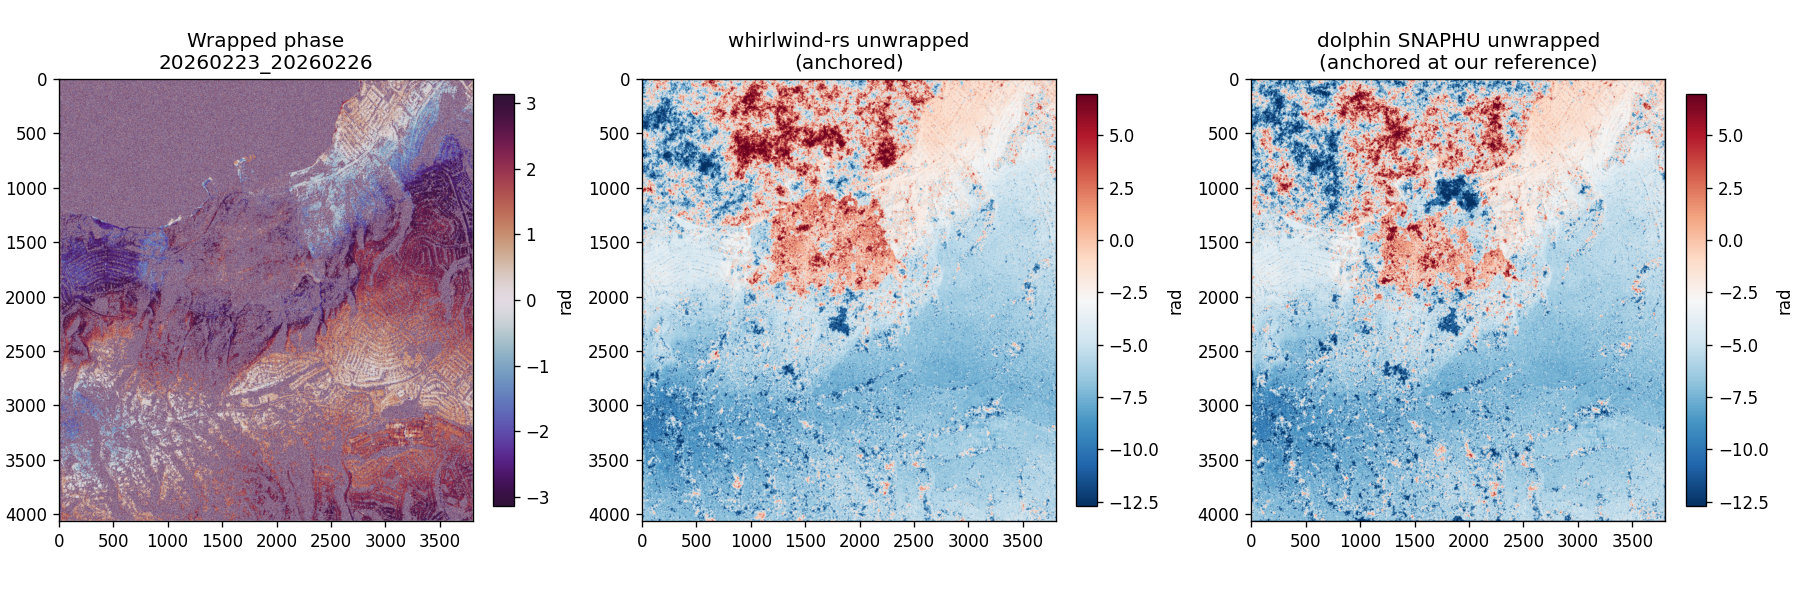
\includegraphics[width=\columnwidth]{fig_palos_verdes_full_wrapped_vs_unwrapped.png}
\caption{Palos Verdes full scene ($4065\times 3802$, 150 IGs, 52 dates):
wrapped phase (left), \texttt{whirlwind-rs} unwrap with the CRLB cost
and the boundary-residue fix (middle), and dolphin's SNAPHU output for
the same IG (right). Both panels share the same colorbar and reference
anchor; the large-scale spatial structure matches across the two
unwrappings.}
\label{fig:full}
\end{figure}

\begin{figure}[t]
\centering

\includegraphics[width=\columnwidth]{fig_palos_verdes_1024_wrapped_vs_unwrapped.png}
\caption{1024² Palos Verdes tile after the boundary-residue fix.
Median absolute RMS to SNAPHU drops from 17.56~rad (before fix) to
2.29~rad (after fix) on this tile; 100\% of pixels match modulo $2\pi$
on every one of the 60 IGs in the stack.}
\label{fig:bdyfix}
\end{figure}

\begin{figure}[t]
\centering
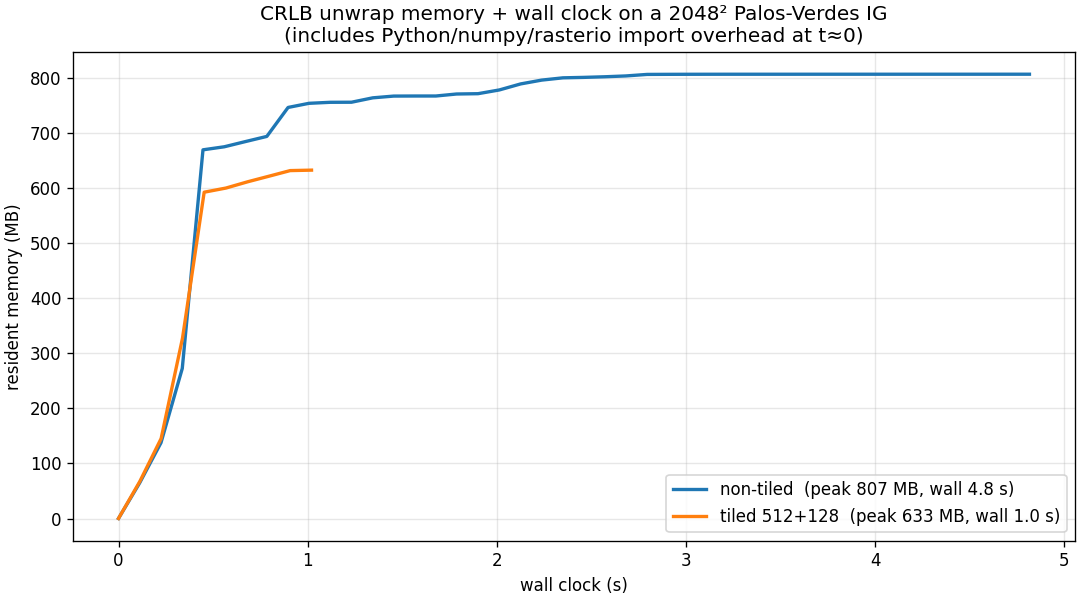
\includegraphics[width=\columnwidth]{fig_tile_memory.png}
\caption{Wall clock and resident memory profile, single $2048^2$ IG.
Non-tiled: 807~MB peak / 4.8~s. Tiled $512+128$: 633~MB peak / 1.0~s.
The tile parallelism is the dominant speedup at this size; the
peak-memory benefit grows quadratically with image side at full scene.}
\label{fig:tile-mem}
\end{figure}

\begin{table}[t]
\centering
\caption{Per-IG agreement with dolphin SNAPHU on Palos Verdes, anchored
at the same reference pixel.}
\label{tab:metrics}
\begin{tabular}{lcc}
\toprule
& 1024² tile, 60 IGs & full scene, 150 IGs \\
\midrule
median \% within $\pi/2$ (mod $2\pi$) & 100.0\,\% & 100.0\,\% \\
median absolute RMS (before bdy fix) & 17.56~rad & 4.72~rad \\
\textbf{median absolute RMS (after fix)} & \textbf{2.29~rad} & \textbf{2.31~rad} \\
IGs with absolute RMS $<1$~rad & 15/60 & 0/150 \\
Stage-1 wall clock (before fix) & 19.2~s & 171~min \\
\textbf{Stage-1 wall clock (after fix)} & \textbf{18.4~s} & \textbf{33~min} \\
\bottomrule
\end{tabular}
\end{table}

Validation is on a Capella stack at Palos Verdes (52 acquisitions,
3--18 day baselines, $4065\times 3802$ pixels, 150 short-baseline IGs).
Phase linking and the SNAPHU baseline are run via the dolphin pipeline
\cite{dolphin}.

% --- Discussion -----------------------------------------------------------

\section{Discussion and Limitations}\label{sec:discussion}

The boundary-residue fix has a single technical claim: the augmented
residue grid is globally charge-balanced by Stokes's theorem, and
without that, MCF on real data with significant boundary-exit
wrap-lines is forced to pair them internally and the snake-path
integration accumulates large integer errors. Its impact is substantial
($7.7\times$ improvement in median absolute RMS on the 1024² tile;
$5\times$ Stage-1 speedup on the full scene from MCF converging in
fewer primal-dual iterations).

We deliberately default the tree-based temporal closure correction
\emph{off}. With the per-IG unwraps now mostly correct, residual
outliers in a few tree edges propagate through the BFS into every
$\theta_d$ downstream of that edge and are rounded onto non-tree edges
incorrectly. A robust closure step --- median-of-multiple-trees,
sparse-network projection, or a true Bayesian per-pixel posterior via
LAMBDA-style weighted integer least squares --- is the natural
next step.

The remaining $\sim 2$~rad median absolute RMS to SNAPHU is real
integer-ambiguity disagreement: both implementations are valid
solutions of the underlying integer-ambiguity problem with different
cost functions and different residual-graph topologies. Downstream
displacement-time-series inversion (SBAS or similar) should agree to
within the noise floor after its own network inversion.

\section*{Software and Reproducibility}

Implementation in Rust with Python bindings is available at
\url{https://github.com/scottstanie/whirlwind-rs}. The shell script
\texttt{scripts/reproduce.sh} runs the full pipeline (Stage 1 + quality
map + dolphin comparison + figure generation) on the 1024² tile in
about 30~s wall clock; \texttt{scripts/reproduce.sh~--full} runs on the
4065$\times$3802 scene in about 33~min.

% --- References -----------------------------------------------------------

\begin{thebibliography}{9}
\bibitem{snaphu}
C.\ W.\ Chen and H.\ A.\ Zebker,
``Phase unwrapping for large SAR interferograms: Statistical segmentation
and generalized network models,''
\emph{IEEE Trans.\ Geosci.\ Remote Sens.}, vol.~40, no.~8,
pp.~1709--1719, 2002.

\bibitem{phaselink-emi}
H.\ Ansari, F.\ De Zan, and A.\ Parizzi,
``Study of systematic bias in measuring surface deformation with SAR
interferometry,''
\emph{IEEE Trans.\ Geosci.\ Remote Sens.}, vol.~59, no.~2,
pp.~1285--1301, 2021.

\bibitem{phaselink-evd}
A.\ Ferretti et al.,
``A new algorithm for processing interferometric data-stacks: SqueeSAR,''
\emph{IEEE Trans.\ Geosci.\ Remote Sens.}, vol.~49, no.~9,
pp.~3460--3470, 2011.

\bibitem{spurt}
\emph{spurt: spatio-temporal unwrapping toolbox.}
\url{https://github.com/isce-framework/spurt}.

\bibitem{lambda}
P.\ J.\ G.\ Teunissen,
``The least-squares ambiguity decorrelation adjustment: a method for fast
GPS integer ambiguity estimation,''
\emph{J.\ Geodesy}, vol.~70, no.~1--2, pp.~65--82, 1995.

\bibitem{carballo}
G.\ F.\ Carballo and P.\ W.\ Fieguth,
``Probabilistic cost functions for network flow phase unwrapping,''
\emph{IEEE Trans.\ Geosci.\ Remote Sens.}, vol.~38, no.~5,
pp.~2192--2201, 2000.

\bibitem{whirlwind}
\emph{Whirlwind: a 2D phase unwrapper (C++).}
\url{https://github.com/isce-framework/whirlwind}.

\bibitem{dolphin}
\emph{dolphin: phase linking and SBAS time-series processing for InSAR.}
\url{https://github.com/isce-framework/dolphin}.

\end{thebibliography}

\end{document}
